\documentclass[twoside]{book}

% Packages required by doxygen
\usepackage{fixltx2e}
\usepackage{calc}
\usepackage{doxygen}
\usepackage[export]{adjustbox} % also loads graphicx
\usepackage{graphicx}
\usepackage[utf8]{inputenc}
\usepackage{makeidx}
\usepackage{multicol}
\usepackage{multirow}
\PassOptionsToPackage{warn}{textcomp}
\usepackage{textcomp}
\usepackage[nointegrals]{wasysym}
\usepackage[table]{xcolor}

% Font selection
\usepackage[T1]{fontenc}
\usepackage[scaled=.90]{helvet}
\usepackage{courier}
\usepackage{amssymb}
\usepackage{sectsty}
\renewcommand{\familydefault}{\sfdefault}
\allsectionsfont{%
  \fontseries{bc}\selectfont%
  \color{darkgray}%
}
\renewcommand{\DoxyLabelFont}{%
  \fontseries{bc}\selectfont%
  \color{darkgray}%
}
\newcommand{\+}{\discretionary{\mbox{\scriptsize$\hookleftarrow$}}{}{}}

% Page & text layout
\usepackage{geometry}
\geometry{%
  a4paper,%
  top=2.5cm,%
  bottom=2.5cm,%
  left=2.5cm,%
  right=2.5cm%
}
\tolerance=750
\hfuzz=15pt
\hbadness=750
\setlength{\emergencystretch}{15pt}
\setlength{\parindent}{0cm}
\setlength{\parskip}{3ex plus 2ex minus 2ex}
\makeatletter
\renewcommand{\paragraph}{%
  \@startsection{paragraph}{4}{0ex}{-1.0ex}{1.0ex}{%
    \normalfont\normalsize\bfseries\SS@parafont%
  }%
}
\renewcommand{\subparagraph}{%
  \@startsection{subparagraph}{5}{0ex}{-1.0ex}{1.0ex}{%
    \normalfont\normalsize\bfseries\SS@subparafont%
  }%
}
\makeatother

% Headers & footers
\usepackage{fancyhdr}
\pagestyle{fancyplain}
\fancyhead[LE]{\fancyplain{}{\bfseries\thepage}}
\fancyhead[CE]{\fancyplain{}{}}
\fancyhead[RE]{\fancyplain{}{\bfseries\leftmark}}
\fancyhead[LO]{\fancyplain{}{\bfseries\rightmark}}
\fancyhead[CO]{\fancyplain{}{}}
\fancyhead[RO]{\fancyplain{}{\bfseries\thepage}}
\fancyfoot[LE]{\fancyplain{}{}}
\fancyfoot[CE]{\fancyplain{}{}}
\fancyfoot[RE]{\fancyplain{}{\bfseries\scriptsize Generated by Doxygen }}
\fancyfoot[LO]{\fancyplain{}{\bfseries\scriptsize Generated by Doxygen }}
\fancyfoot[CO]{\fancyplain{}{}}
\fancyfoot[RO]{\fancyplain{}{}}
\renewcommand{\footrulewidth}{0.4pt}
\renewcommand{\chaptermark}[1]{%
  \markboth{#1}{}%
}
\renewcommand{\sectionmark}[1]{%
  \markright{\thesection\ #1}%
}

% Indices & bibliography
\usepackage{natbib}
\usepackage[titles]{tocloft}
\setcounter{tocdepth}{3}
\setcounter{secnumdepth}{5}
\makeindex

% Hyperlinks (required, but should be loaded last)
\usepackage{ifpdf}
\ifpdf
  \usepackage[pdftex,pagebackref=true]{hyperref}
\else
  \usepackage[ps2pdf,pagebackref=true]{hyperref}
\fi
\hypersetup{%
  colorlinks=true,%
  linkcolor=blue,%
  citecolor=blue,%
  unicode%
}

% Custom commands
\newcommand{\clearemptydoublepage}{%
  \newpage{\pagestyle{empty}\cleardoublepage}%
}

\usepackage{caption}
\captionsetup{labelsep=space,justification=centering,font={bf},singlelinecheck=off,skip=4pt,position=top}

%===== C O N T E N T S =====

\begin{document}

% Titlepage & ToC
\hypersetup{pageanchor=false,
             bookmarksnumbered=true,
             pdfencoding=unicode
            }
\pagenumbering{roman}
\begin{titlepage}
\vspace*{7cm}
\begin{center}%
{\Large My Project }\\
\vspace*{1cm}
{\large Generated by Doxygen 1.8.11}\\
\end{center}
\end{titlepage}
\clearemptydoublepage
\tableofcontents
\clearemptydoublepage
\pagenumbering{arabic}
\hypersetup{pageanchor=true}

%--- Begin generated contents ---
\chapter{File Index}
\section{File List}
Here is a list of all documented files with brief descriptions\-:\begin{DoxyCompactList}
\item\contentsline{section}{\hyperlink{BGField1_8hh}{B\-G\-Field1.\-hh} \\*B\-G\-Field1-\/7 are 7 almost identical headers that define 7 similar classes derived from \char`\"{}\-E\-M\-M\-A\-Element\-Field.\-hh.\char`\"{} They each descibe an E\-M field that is part of E\-M\-M\-A }{\pageref{BGField1_8hh}}{}
\item\contentsline{section}{\hyperlink{BGField2_8hh}{B\-G\-Field2.\-hh} \\*B\-G\-Field1-\/7 are 7 almost identical headers that define 7 similar classes derived from \char`\"{}\-E\-M\-M\-A\-Element\-Field.\-hh.\char`\"{} They each descibe an E\-M field that is part of E\-M\-M\-A }{\pageref{BGField2_8hh}}{}
\item\contentsline{section}{\hyperlink{BGField3_8hh}{B\-G\-Field3.\-hh} \\*B\-G\-Field1-\/7 are 7 almost identical headers that define 7 similar classes derived from \char`\"{}\-E\-M\-M\-A\-Element\-Field.\-hh.\char`\"{} They each descibe an E\-M field that is part of E\-M\-M\-A }{\pageref{BGField3_8hh}}{}
\item\contentsline{section}{\hyperlink{BGField4_8hh}{B\-G\-Field4.\-hh} \\*B\-G\-Field1-\/7 are 7 almost identical headers that define 7 similar classes derived from \char`\"{}\-E\-M\-M\-A\-Element\-Field.\-hh.\char`\"{} They each descibe an E\-M field that is part of E\-M\-M\-A }{\pageref{BGField4_8hh}}{}
\item\contentsline{section}{\hyperlink{BGField5_8hh}{B\-G\-Field5.\-hh} \\*B\-G\-Field1-\/7 are 7 almost identical headers that define 7 similar classes derived from \char`\"{}\-E\-M\-M\-A\-Element\-Field.\-hh.\char`\"{} They each descibe an E\-M field that is part of E\-M\-M\-A }{\pageref{BGField5_8hh}}{}
\item\contentsline{section}{\hyperlink{BGField6_8hh}{B\-G\-Field6.\-hh} \\*B\-G\-Field1-\/7 are 7 almost identical headers that define 7 similar classes derived from \char`\"{}\-E\-M\-M\-A\-Element\-Field.\-hh.\char`\"{} They each descibe an E\-M field that is part of E\-M\-M\-A }{\pageref{BGField6_8hh}}{}
\item\contentsline{section}{\hyperlink{BGField7_8hh}{B\-G\-Field7.\-hh} \\*B\-G\-Field1-\/7 are 7 almost identical headers that define 7 similar classes derived from \char`\"{}\-E\-M\-M\-A\-Element\-Field.\-hh.\char`\"{} They each descibe an E\-M field that is part of E\-M\-M\-A }{\pageref{BGField7_8hh}}{}
\item\contentsline{section}{\hyperlink{c2__factory_8hh}{c2\-\_\-factory.\-hh} \\*Provides a factory class to avoid an infinite number of template declarations }{\pageref{c2__factory_8hh}}{}
\item\contentsline{section}{\hyperlink{c2__function_8hh}{c2\-\_\-function.\-hh} \\*Provides the headers for the general \hyperlink{classc2__function}{c2\-\_\-function} algebra which supports fast, flexible operations on piecewise-\/twice-\/differentiable functions }{\pageref{c2__function_8hh}}{}
\item\contentsline{section}{\hyperlink{CathodeWireParameterisation_8hh}{Cathode\-Wire\-Parameterisation.\-hh} \\*This is a parameterisation that describes a series of cylinders (wires) along X }{\pageref{CathodeWireParameterisation_8hh}}{}
\item\contentsline{section}{\hyperlink{EMFieldDebugger_8hh}{E\-M\-Field\-Debugger.\-hh} \\*This header declares a class used in the corresponding source file that calculates the value of E\-M fields at different locations in the simulation }{\pageref{EMFieldDebugger_8hh}}{}
\item\contentsline{section}{\hyperlink{EMMAAnalysisManager_8hh}{E\-M\-M\-A\-Analysis\-Manager.\-hh} \\*This header calls upon several root files and declares other functions for a source file. These functions call upon and write to R\-O\-O\-T files to display simulation outcomes or results }{\pageref{EMMAAnalysisManager_8hh}}{}
\item\contentsline{section}{\hyperlink{EMMADetectorConstMessenger_8hh}{E\-M\-M\-A\-Detector\-Const\-Messenger.\-hh} \\*This header file contains deals with user commands relating to detector construction }{\pageref{EMMADetectorConstMessenger_8hh}}{}
\item\contentsline{section}{\hyperlink{EMMADetectorConstruction_8hh}{E\-M\-M\-A\-Detector\-Construction.\-hh} \\*This header file builds on the G4 header \char`\"{}\-G4\-V\-User\-Detector\-Construction.\-hh\char`\"{} to set the global G4 variables specifying the materials and simulation attributes of the E\-M\-M\-A detectors. Several E\-M\-M\-A functions (regarding its detectors) are also defined }{\pageref{EMMADetectorConstruction_8hh}}{}
\item\contentsline{section}{\hyperlink{EMMADriftChamber_8hh}{E\-M\-M\-A\-Drift\-Chamber.\-hh} \\*This header contains the class required to run the P\-G\-A\-C drift chamber (see also G4\-Sensitive\-Detector.\-hh) }{\pageref{EMMADriftChamber_8hh}}{}
\item\contentsline{section}{\hyperlink{EMMADriftChamberHit_8hh}{E\-M\-M\-A\-Drift\-Chamber\-Hit.\-hh} \\*This class manages the hit object in regards to the drift chamber part of the simulation. It defines global variables and functions for the G4 code to run necessary hit simulations. The virtual methods draw() and print() are used. For further details about each part of this file, examine the accompanying explanations adjacent to the classes }{\pageref{EMMADriftChamberHit_8hh}}{}
\item\contentsline{section}{\hyperlink{EMMAElementField_8hh}{E\-M\-M\-A\-Element\-Field.\-hh} \\*This is the interface class used by Global\-Field to compute the field value at a given point\mbox{[}\mbox{]} }{\pageref{EMMAElementField_8hh}}{}
\item\contentsline{section}{\hyperlink{EMMAEMPhysics_8hh}{E\-M\-M\-A\-E\-M\-Physics.\-hh} \\*The G4 header \char`\"{}\-G4\-V\-Physics\-Constructor.\-hh\char`\"{} contains a virtual class that must be used to create concrete classes for specific applications (such as E\-M\-M\-A). This header builds such a concrete class to include E\-M\-M\-A's specific particles and processes. Specifically, this header defines particles and processes required to simulate E\-M interactions }{\pageref{EMMAEMPhysics_8hh}}{}
\item\contentsline{section}{\hyperlink{EMMAEventAction_8hh}{E\-M\-M\-A\-Event\-Action.\-hh} \\*This header defines the user's action class, and specifically, the beginning and end of a user action. It generates from the Primary\-Generator headers as the user begins an action. Contains functions that are invoked by G4\-Event\-Manager }{\pageref{EMMAEventAction_8hh}}{}
\item\contentsline{section}{\hyperlink{EMMAEventActionMessenger_8hh}{E\-M\-M\-A\-Event\-Action\-Messenger.\-hh} \\*This file is responsible for deleting commands, delivering commands to destination classes, defining global G4 variables specific to E\-M\-M\-A, and replying the current values of the parameters (again as described the \char`\"{}\-G4\-U\-Imessenger.\-hh\char`\"{} source file) regarding the event action (from the primary generator) }{\pageref{EMMAEventActionMessenger_8hh}}{}
\item\contentsline{section}{\hyperlink{EMMAGeneralPhysics_8hh}{E\-M\-M\-A\-General\-Physics.\-hh} \\*This header defines particles and processes required for other more specific physics processes }{\pageref{EMMAGeneralPhysics_8hh}}{}
\item\contentsline{section}{\hyperlink{EMMAGlobalField_8hh}{E\-M\-M\-A\-Global\-Field.\-hh} \\*Handles the global Electro\-Magnetic field }{\pageref{EMMAGlobalField_8hh}}{}
\item\contentsline{section}{\hyperlink{EMMAHadronPhysics_8hh}{E\-M\-M\-A\-Hadron\-Physics.\-hh} \\*The G4 header \char`\"{}\-G4\-V\-Physics\-Constructor.\-hh\char`\"{} contains a virtual class that must be used to create concrete classes for specific applications (such as E\-M\-M\-A). Specifically, this header defines particles and processes required to simulate hadron interactions }{\pageref{EMMAHadronPhysics_8hh}}{}
\item\contentsline{section}{\hyperlink{EMMAIonChamber_8hh}{E\-M\-M\-A\-Ion\-Chamber.\-hh} \\*This defines a calorimeter sensitive detector class (ion chamber). Uses the inherited G4 detector construction classes to build the operation of the ion chamber }{\pageref{EMMAIonChamber_8hh}}{}
\item\contentsline{section}{\hyperlink{EMMAIonChamberHit_8hh}{E\-M\-M\-A\-Ion\-Chamber\-Hit.\-hh} \\*Calorimeter (ion chamber) hit class\-: defines data members to store the the energy deposit and track lengths of charged particles in a selected volume }{\pageref{EMMAIonChamberHit_8hh}}{}
\item\contentsline{section}{\hyperlink{EMMAIonPhysics_8hh}{E\-M\-M\-A\-Ion\-Physics.\-hh} \\*The G4 header \char`\"{}\-G4\-V\-Physics\-Constructor.\-hh\char`\"{} contains a virtual class that must be used to create concrete classes for specific applications (such as E\-M\-M\-A). Specifically, this header defines particles and processes required to simulate ion interactions }{\pageref{EMMAIonPhysics_8hh}}{}
\item\contentsline{section}{\hyperlink{EMMAIonPhysicsMessenger_8hh}{E\-M\-M\-A\-Ion\-Physics\-Messenger.\-hh} \\*This header file contains deals with user commands relating to ionic physics processes }{\pageref{EMMAIonPhysicsMessenger_8hh}}{}
\item\contentsline{section}{\hyperlink{EMMAMuonPhysics_8hh}{E\-M\-M\-A\-Muon\-Physics.\-hh} \\*The G4 header \char`\"{}\-G4\-V\-Physics\-Constructor.\-hh\char`\"{} contains a virtual class that must be used to create concrete classes for specific applications (such as E\-M\-M\-A). Specifically, this header defines particles and processes required to simulate muon interactions }{\pageref{EMMAMuonPhysics_8hh}}{}
\item\contentsline{section}{\hyperlink{EMMANuclearReactionDataSet_8hh}{E\-M\-M\-A\-Nuclear\-Reaction\-Data\-Set.\-hh} \\*Data set for (two body) nuclear reaction cross sections. Inherited from similar G4 headers }{\pageref{EMMANuclearReactionDataSet_8hh}}{}
\item\contentsline{section}{\hyperlink{EMMANuclearReactionProcess_8hh}{E\-M\-M\-A\-Nuclear\-Reaction\-Process.\-hh} \\*Nuclear-\/reaction process for projectile (Z1,A1) striking target (Z2,A2) with cross section (cs) }{\pageref{EMMANuclearReactionProcess_8hh}}{}
\item\contentsline{section}{\hyperlink{EMMANuclearReactionTwoBody_8hh}{E\-M\-M\-A\-Nuclear\-Reaction\-Two\-Body.\-hh} \\*Nuclear-\/reaction model for two-\/body final-\/state (Z3,A3)+(Z4,A4) after a two body reaction between a projectile and target }{\pageref{EMMANuclearReactionTwoBody_8hh}}{}
\item\contentsline{section}{\hyperlink{EMMAPhysicsList_8hh}{E\-M\-M\-A\-Physics\-List.\-hh} \\*E\-M\-M\-A's specific objects and particles are registered from the virtual class in \char`\"{}\-G4\-V\-Physics\-Constructor.\-hh.\char`\"{} These objects are registered to G4\-User\-Physics\-List, which is the parent of \char`\"{}\-G4\-V\-Modular\-Physics\-List.\-hh.\char`\"{} This header defines a concrete class inherited from \char`\"{}\-G4\-V\-Modular\-Physics\-List.\-hh\char`\"{} }{\pageref{EMMAPhysicsList_8hh}}{}
\item\contentsline{section}{\hyperlink{EMMAPrimaryGeneratorAction_8hh}{E\-M\-M\-A\-Primary\-Generator\-Action.\-hh} \\*This is an important class responsible for primary particle or vertex generation. It is required by G4; the Primary Generator is not an actual physical component of E\-M\-M\-A but rather a G4 construction element. This class is the concrete class stemming from the virtual class found in \char`\"{}\-G4\-V\-User\-Primary\-Generator\-Action.\-hh.\char`\"{} }{\pageref{EMMAPrimaryGeneratorAction_8hh}}{}
\item\contentsline{section}{\hyperlink{EMMAPrimaryGeneratorMessenger_8hh}{E\-M\-M\-A\-Primary\-Generator\-Messenger.\-hh} \\*This file is responsible for deleting commands, delivering commands to destination classes, defining global G4 variables specific to E\-M\-M\-A, and replying the current values of the parameters (again as described the \char`\"{}\-G4\-U\-Imessenger.\-hh\char`\"{} source file) regarding the primary generator (of the events) }{\pageref{EMMAPrimaryGeneratorMessenger_8hh}}{}
\item\contentsline{section}{\hyperlink{EMMASteppingAction_8hh}{E\-M\-M\-A\-Stepping\-Action.\-hh} \\*Headers that have to do with \char`\"{}stepping\char`\"{} (loops) is related to tracking the particle and its interactions with its surroundings. This class defines functions that build on \char`\"{}\-G4\-User\-Stepping\-Action.\-hh,\char`\"{} which represents user actions during \char`\"{}stepping.\char`\"{} }{\pageref{EMMASteppingAction_8hh}}{}
\item\contentsline{section}{\hyperlink{EMMASteppingVerbose_8hh}{E\-M\-M\-A\-Stepping\-Verbose.\-hh} \\*This class manages the verbose outputs in G4\-Stepping\-Manager. It shows how to extract information during the tracking of a particle }{\pageref{EMMASteppingVerbose_8hh}}{}
\item\contentsline{section}{\hyperlink{F04StepMax_8hh}{F04\-Step\-Max.\-hh} \\*Header defines a class relating to the step (tracking) of a particle involved in a discrete process. For more general information see this header's dependencies }{\pageref{F04StepMax_8hh}}{}
\item\contentsline{section}{\hyperlink{G4LindhardPartition_8hh}{G4\-Lindhard\-Partition.\-hh} \\*A seemingly periphery code that calculates the non-\/ionizing energy loss of radiation via the Lindhard partition function. Used to calculate energy deposited in target by the beam thereby affecting energy of recoils }{\pageref{G4LindhardPartition_8hh}}{}
\item\contentsline{section}{\hyperlink{G4ScreenedNuclearRecoil_8hh}{G4\-Screened\-Nuclear\-Recoil.\-hh} \\*Builds the process of screened electromagnetic nuclear elastic scattering. Declares many functions primarily used for coulomb interactions between nuclei }{\pageref{G4ScreenedNuclearRecoil_8hh}}{}
\item\contentsline{section}{\hyperlink{PGACWireParameterisation_8hh}{P\-G\-A\-C\-Wire\-Parameterisation.\-hh} \\*A parameterisation that describes a series of cylinders along Z (the wires in the P\-C\-A\-G ioin drift chamber) }{\pageref{PGACWireParameterisation_8hh}}{}
\item\contentsline{section}{\hyperlink{SpectrometerConstruction_8hh}{Spectrometer\-Construction.\-hh} \\*Builds the E\-M\-M\-A spectrometer through defining classes and variables, including those for slit control. This header is built upon the virtual classes inherited from \char`\"{}\-G4\-V\-User\-Detector\-Construction.\-hh.\char`\"{} }{\pageref{SpectrometerConstruction_8hh}}{}
\item\contentsline{section}{{\bfseries Stacking\-Action.\-hh} }{\pageref{StackingAction_8hh}}{}
\item\contentsline{section}{{\bfseries Tracking\-Action.\-hh} }{\pageref{TrackingAction_8hh}}{}
\end{DoxyCompactList}

\chapter{File Documentation}
\hypertarget{CMakeLists_8txt}{}\section{C\+Make\+Lists.\+txt File Reference}
\label{CMakeLists_8txt}\index{C\+Make\+Lists.\+txt@{C\+Make\+Lists.\+txt}}
\subsection*{Functions}
\begin{DoxyCompactItemize}
\item 
\hyperlink{CMakeLists_8txt_a96d513d95f99c6a7d814bc5219aa207a}{cmake\+\_\+minimum\+\_\+required} (V\+E\+R\+S\+I\+ON 2.\+6 F\+A\+T\+A\+L\+\_\+\+E\+R\+R\+OR) project(E\+M\+MA) option(W\+I\+T\+H\+\_\+\+G\+E\+A\+N\+T4\+\_\+\+U\+I\+V\+IS\char`\"{}Build example with Geant4 UI and Vis drivers\char`\"{}ON) if(W\+I\+T\+H\+\_\+\+G\+E\+A\+N\+T4\+\_\+\+U\+I\+V\+IS) \hyperlink{CMakeLists_8txt_ac8b9ea4be7802858ed602bf5474e31b4}{find\+\_\+package}(Geant4 R\+E\+Q\+U\+I\+R\+ED ui\+\_\+all vis\+\_\+all) else() \hyperlink{CMakeLists_8txt_ac8b9ea4be7802858ed602bf5474e31b4}{find\+\_\+package}(Geant4 R\+E\+Q\+U\+I\+R\+ED) endif() include(\$
\item 
\hyperlink{CMakeLists_8txt_ac8b9ea4be7802858ed602bf5474e31b4}{find\+\_\+package} (R\+O\+OT) if(R\+O\+O\+T\+\_\+\+F\+O\+U\+ND) add\+\_\+definitions(-\/D\+G4\+A\+N\+A\+L\+Y\+S\+I\+S\+\_\+\+U\+SE) endif() include\+\_\+directories(\$
\end{DoxyCompactItemize}


\subsection{Function Documentation}
\index{C\+Make\+Lists.\+txt@{C\+Make\+Lists.\+txt}!cmake\+\_\+minimum\+\_\+required@{cmake\+\_\+minimum\+\_\+required}}
\index{cmake\+\_\+minimum\+\_\+required@{cmake\+\_\+minimum\+\_\+required}!C\+Make\+Lists.\+txt@{C\+Make\+Lists.\+txt}}
\subsubsection[{\texorpdfstring{cmake\+\_\+minimum\+\_\+required(\+V\+E\+R\+S\+I\+O\+N 2.\+6 F\+A\+T\+A\+L\+\_\+\+E\+R\+R\+O\+R) project(\+E\+M\+M\+A) option(\+W\+I\+T\+H\+\_\+\+G\+E\+A\+N\+T4\+\_\+\+U\+I\+V\+IS""Build example with Geant4 U\+I and Vis drivers""O\+N) if(\+W\+I\+T\+H\+\_\+\+G\+E\+A\+N\+T4\+\_\+\+U\+I\+V\+I\+S) find\+\_\+package(\+Geant4 R\+E\+Q\+U\+I\+R\+E\+D ui\+\_\+all vis\+\_\+all) else() find\+\_\+package(\+Geant4 R\+E\+Q\+U\+I\+R\+E\+D) endif() include(\$}{cmake_minimum_required(VERSION 2.6 FATAL_ERROR) project(EMMA) option(WITH_GEANT4_UIVIS"Build example with Geant4 UI and Vis drivers"ON) if(WITH_GEANT4_UIVIS) find_package(Geant4 REQUIRED ui_all vis_all) else() find_package(Geant4 REQUIRED) endif() include($}}]{\setlength{\rightskip}{0pt plus 5cm}cmake\+\_\+minimum\+\_\+required (
\begin{DoxyParamCaption}
\item[{V\+E\+R\+S\+I\+ON 2.\+6}]{F\+A\+T\+A\+L\+\_\+\+E\+R\+R\+OR}
\end{DoxyParamCaption}
)}\hypertarget{CMakeLists_8txt_a96d513d95f99c6a7d814bc5219aa207a}{}\label{CMakeLists_8txt_a96d513d95f99c6a7d814bc5219aa207a}
\index{C\+Make\+Lists.\+txt@{C\+Make\+Lists.\+txt}!find\+\_\+package@{find\+\_\+package}}
\index{find\+\_\+package@{find\+\_\+package}!C\+Make\+Lists.\+txt@{C\+Make\+Lists.\+txt}}
\subsubsection[{\texorpdfstring{find\+\_\+package(\+R\+O\+O\+T) if(\+R\+O\+O\+T\+\_\+\+F\+O\+U\+N\+D) add\+\_\+definitions(-\/\+D\+G4\+A\+N\+A\+L\+Y\+S\+I\+S\+\_\+\+U\+S\+E) endif() include\+\_\+directories(\$}{find_package(ROOT) if(ROOT_FOUND) add_definitions(-DG4ANALYSIS_USE) endif() include_directories($}}]{\setlength{\rightskip}{0pt plus 5cm}find\+\_\+package (
\begin{DoxyParamCaption}
\item[{R\+O\+OT}]{}
\end{DoxyParamCaption}
)}\hypertarget{CMakeLists_8txt_ac8b9ea4be7802858ed602bf5474e31b4}{}\label{CMakeLists_8txt_ac8b9ea4be7802858ed602bf5474e31b4}

\hypertarget{EMMAapp_8cc}{}\section{E\+M\+M\+Aapp.\+cc File Reference}
\label{EMMAapp_8cc}\index{E\+M\+M\+Aapp.\+cc@{E\+M\+M\+Aapp.\+cc}}
{\ttfamily \#include \char`\"{}G4\+Run\+Manager.\+hh\char`\"{}}\\*
{\ttfamily \#include \char`\"{}G4\+U\+Imanager.\+hh\char`\"{}}\\*
{\ttfamily \#include \char`\"{}E\+M\+M\+A\+Detector\+Construction.\+hh\char`\"{}}\\*
{\ttfamily \#include \char`\"{}E\+M\+M\+A\+Physics\+List.\+hh\char`\"{}}\\*
{\ttfamily \#include \char`\"{}E\+M\+M\+A\+Primary\+Generator\+Action.\+hh\char`\"{}}\\*
{\ttfamily \#include \char`\"{}E\+M\+M\+A\+Event\+Action.\+hh\char`\"{}}\\*
{\ttfamily \#include \char`\"{}E\+M\+M\+A\+Stepping\+Action.\+hh\char`\"{}}\\*
{\ttfamily \#include \char`\"{}E\+M\+M\+A\+Stepping\+Verbose.\+hh\char`\"{}}\\*
{\ttfamily \#include \char`\"{}Tracking\+Action.\+hh\char`\"{}}\\*
{\ttfamily \#include \char`\"{}Stacking\+Action.\+hh\char`\"{}}\\*
{\ttfamily \#include \char`\"{}G4\+Event.\+hh\char`\"{}}\\*
{\ttfamily \#include $<$string$>$}\\*
{\ttfamily \#include $<$fstream$>$}\\*
{\ttfamily \#include $<$sstream$>$}\\*
Include dependency graph for E\+M\+M\+Aapp.\+cc\+:
\nopagebreak
\begin{figure}[H]
\begin{center}
\leavevmode
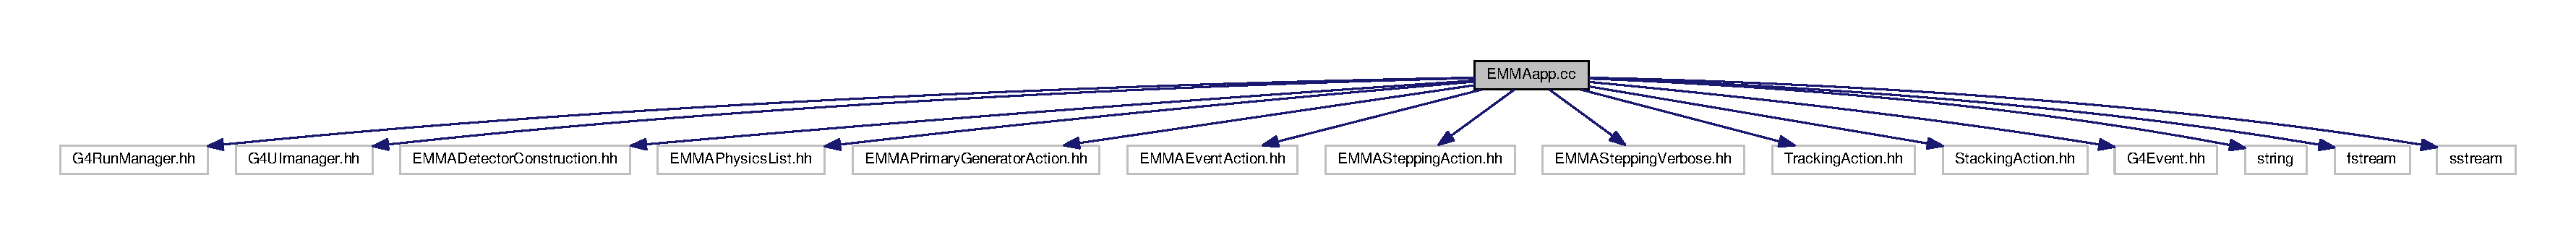
\includegraphics[width=350pt]{EMMAapp_8cc__incl}
\end{center}
\end{figure}
\subsection*{Functions}
\begin{DoxyCompactItemize}
\item 
void \hyperlink{EMMAapp_8cc_a9c3d1609dab49b55541e7a55935dec66}{Read\+User\+Input\+\_\+\+Beam} (G4\+String \&s1, G4\+String \&s2, G4\+String \&s3, G4\+String \&s4, G4\+String \&s5, G4\+String \&s6, G4\+String \&s7, G4\+String \&s8)
\item 
void \hyperlink{EMMAapp_8cc_a243acf7fbf6807f825e460762776e7c5}{Read\+User\+Input\+\_\+\+Reaction} (G4\+String \&s1, G4\+String \&s2, G4\+String \&s3, G4\+String \&s4, G4\+String \&s5, G4\+String \&s6, G4\+String \&s7, G4\+String \&s8, G4\+String \&s9, G4\+String \&s10, G4\+String \&s11, G4\+String \&s12, G4double \&s13)
\item 
void \hyperlink{EMMAapp_8cc_aff2065a5a30dacccfa52f346dbf4586c}{Read\+User\+Input\+\_\+\+Central\+Trajectory} (G4\+String \&s1, G4\+String \&s2, G4\+String \&s3, G4\+String \&s4)
\item 
int \hyperlink{EMMAapp_8cc_a3c04138a5bfe5d72780bb7e82a18e627}{main} (int argc, char $\ast$$\ast$argv)
\end{DoxyCompactItemize}
\subsection*{Variables}
\begin{DoxyCompactItemize}
\item 
G4\+String \hyperlink{EMMAapp_8cc_a28a3faf9b4768b420044f0d81fa645b7}{Mother\+Dir}
\item 
G4\+String \hyperlink{EMMAapp_8cc_a8558631b93942e4ae79b3feb21c97c8f}{User\+Dir}
\item 
G4int \hyperlink{EMMAapp_8cc_a9692863287fc6c571e3d80523f52aaec}{N\+O\+Hslits1} =0
\item 
G4int \hyperlink{EMMAapp_8cc_a5a1b8ea664140faf390f322e99ff9eae}{N\+O\+Hslits2} =0
\item 
G4int \hyperlink{EMMAapp_8cc_acd5e5641cf42ac1ee6029f01552f1242}{N\+O\+Hslits3} =0
\item 
G4int \hyperlink{EMMAapp_8cc_a2999d2feb52b63936e73e99587a94643}{N\+O\+Hslits4} =0
\end{DoxyCompactItemize}


\subsection{Function Documentation}
\index{E\+M\+M\+Aapp.\+cc@{E\+M\+M\+Aapp.\+cc}!main@{main}}
\index{main@{main}!E\+M\+M\+Aapp.\+cc@{E\+M\+M\+Aapp.\+cc}}
\subsubsection[{\texorpdfstring{main(int argc, char $\ast$$\ast$argv)}{main(int argc, char **argv)}}]{\setlength{\rightskip}{0pt plus 5cm}int main (
\begin{DoxyParamCaption}
\item[{int}]{argc, }
\item[{char $\ast$$\ast$}]{argv}
\end{DoxyParamCaption}
)}\hypertarget{EMMAapp_8cc_a3c04138a5bfe5d72780bb7e82a18e627}{}\label{EMMAapp_8cc_a3c04138a5bfe5d72780bb7e82a18e627}
\index{E\+M\+M\+Aapp.\+cc@{E\+M\+M\+Aapp.\+cc}!Read\+User\+Input\+\_\+\+Beam@{Read\+User\+Input\+\_\+\+Beam}}
\index{Read\+User\+Input\+\_\+\+Beam@{Read\+User\+Input\+\_\+\+Beam}!E\+M\+M\+Aapp.\+cc@{E\+M\+M\+Aapp.\+cc}}
\subsubsection[{\texorpdfstring{Read\+User\+Input\+\_\+\+Beam(\+G4\+String \&s1, G4\+String \&s2, G4\+String \&s3, G4\+String \&s4, G4\+String \&s5, G4\+String \&s6, G4\+String \&s7, G4\+String \&s8)}{ReadUserInput_Beam(G4String &s1, G4String &s2, G4String &s3, G4String &s4, G4String &s5, G4String &s6, G4String &s7, G4String &s8)}}]{\setlength{\rightskip}{0pt plus 5cm}void Read\+User\+Input\+\_\+\+Beam (
\begin{DoxyParamCaption}
\item[{G4\+String \&}]{s1, }
\item[{G4\+String \&}]{s2, }
\item[{G4\+String \&}]{s3, }
\item[{G4\+String \&}]{s4, }
\item[{G4\+String \&}]{s5, }
\item[{G4\+String \&}]{s6, }
\item[{G4\+String \&}]{s7, }
\item[{G4\+String \&}]{s8}
\end{DoxyParamCaption}
)}\hypertarget{EMMAapp_8cc_a9c3d1609dab49b55541e7a55935dec66}{}\label{EMMAapp_8cc_a9c3d1609dab49b55541e7a55935dec66}
\index{E\+M\+M\+Aapp.\+cc@{E\+M\+M\+Aapp.\+cc}!Read\+User\+Input\+\_\+\+Central\+Trajectory@{Read\+User\+Input\+\_\+\+Central\+Trajectory}}
\index{Read\+User\+Input\+\_\+\+Central\+Trajectory@{Read\+User\+Input\+\_\+\+Central\+Trajectory}!E\+M\+M\+Aapp.\+cc@{E\+M\+M\+Aapp.\+cc}}
\subsubsection[{\texorpdfstring{Read\+User\+Input\+\_\+\+Central\+Trajectory(\+G4\+String \&s1, G4\+String \&s2, G4\+String \&s3, G4\+String \&s4)}{ReadUserInput_CentralTrajectory(G4String &s1, G4String &s2, G4String &s3, G4String &s4)}}]{\setlength{\rightskip}{0pt plus 5cm}void Read\+User\+Input\+\_\+\+Central\+Trajectory (
\begin{DoxyParamCaption}
\item[{G4\+String \&}]{s1, }
\item[{G4\+String \&}]{s2, }
\item[{G4\+String \&}]{s3, }
\item[{G4\+String \&}]{s4}
\end{DoxyParamCaption}
)}\hypertarget{EMMAapp_8cc_aff2065a5a30dacccfa52f346dbf4586c}{}\label{EMMAapp_8cc_aff2065a5a30dacccfa52f346dbf4586c}
\index{E\+M\+M\+Aapp.\+cc@{E\+M\+M\+Aapp.\+cc}!Read\+User\+Input\+\_\+\+Reaction@{Read\+User\+Input\+\_\+\+Reaction}}
\index{Read\+User\+Input\+\_\+\+Reaction@{Read\+User\+Input\+\_\+\+Reaction}!E\+M\+M\+Aapp.\+cc@{E\+M\+M\+Aapp.\+cc}}
\subsubsection[{\texorpdfstring{Read\+User\+Input\+\_\+\+Reaction(\+G4\+String \&s1, G4\+String \&s2, G4\+String \&s3, G4\+String \&s4, G4\+String \&s5, G4\+String \&s6, G4\+String \&s7, G4\+String \&s8, G4\+String \&s9, G4\+String \&s10, G4\+String \&s11, G4\+String \&s12, G4double \&s13)}{ReadUserInput_Reaction(G4String &s1, G4String &s2, G4String &s3, G4String &s4, G4String &s5, G4String &s6, G4String &s7, G4String &s8, G4String &s9, G4String &s10, G4String &s11, G4String &s12, G4double &s13)}}]{\setlength{\rightskip}{0pt plus 5cm}void Read\+User\+Input\+\_\+\+Reaction (
\begin{DoxyParamCaption}
\item[{G4\+String \&}]{s1, }
\item[{G4\+String \&}]{s2, }
\item[{G4\+String \&}]{s3, }
\item[{G4\+String \&}]{s4, }
\item[{G4\+String \&}]{s5, }
\item[{G4\+String \&}]{s6, }
\item[{G4\+String \&}]{s7, }
\item[{G4\+String \&}]{s8, }
\item[{G4\+String \&}]{s9, }
\item[{G4\+String \&}]{s10, }
\item[{G4\+String \&}]{s11, }
\item[{G4\+String \&}]{s12, }
\item[{G4double \&}]{s13}
\end{DoxyParamCaption}
)}\hypertarget{EMMAapp_8cc_a243acf7fbf6807f825e460762776e7c5}{}\label{EMMAapp_8cc_a243acf7fbf6807f825e460762776e7c5}


\subsection{Variable Documentation}
\index{E\+M\+M\+Aapp.\+cc@{E\+M\+M\+Aapp.\+cc}!Mother\+Dir@{Mother\+Dir}}
\index{Mother\+Dir@{Mother\+Dir}!E\+M\+M\+Aapp.\+cc@{E\+M\+M\+Aapp.\+cc}}
\subsubsection[{\texorpdfstring{Mother\+Dir}{MotherDir}}]{\setlength{\rightskip}{0pt plus 5cm}G4\+String Mother\+Dir}\hypertarget{EMMAapp_8cc_a28a3faf9b4768b420044f0d81fa645b7}{}\label{EMMAapp_8cc_a28a3faf9b4768b420044f0d81fa645b7}
\index{E\+M\+M\+Aapp.\+cc@{E\+M\+M\+Aapp.\+cc}!N\+O\+Hslits1@{N\+O\+Hslits1}}
\index{N\+O\+Hslits1@{N\+O\+Hslits1}!E\+M\+M\+Aapp.\+cc@{E\+M\+M\+Aapp.\+cc}}
\subsubsection[{\texorpdfstring{N\+O\+Hslits1}{NOHslits1}}]{\setlength{\rightskip}{0pt plus 5cm}G4int N\+O\+Hslits1 =0}\hypertarget{EMMAapp_8cc_a9692863287fc6c571e3d80523f52aaec}{}\label{EMMAapp_8cc_a9692863287fc6c571e3d80523f52aaec}
\index{E\+M\+M\+Aapp.\+cc@{E\+M\+M\+Aapp.\+cc}!N\+O\+Hslits2@{N\+O\+Hslits2}}
\index{N\+O\+Hslits2@{N\+O\+Hslits2}!E\+M\+M\+Aapp.\+cc@{E\+M\+M\+Aapp.\+cc}}
\subsubsection[{\texorpdfstring{N\+O\+Hslits2}{NOHslits2}}]{\setlength{\rightskip}{0pt plus 5cm}G4int N\+O\+Hslits2 =0}\hypertarget{EMMAapp_8cc_a5a1b8ea664140faf390f322e99ff9eae}{}\label{EMMAapp_8cc_a5a1b8ea664140faf390f322e99ff9eae}
\index{E\+M\+M\+Aapp.\+cc@{E\+M\+M\+Aapp.\+cc}!N\+O\+Hslits3@{N\+O\+Hslits3}}
\index{N\+O\+Hslits3@{N\+O\+Hslits3}!E\+M\+M\+Aapp.\+cc@{E\+M\+M\+Aapp.\+cc}}
\subsubsection[{\texorpdfstring{N\+O\+Hslits3}{NOHslits3}}]{\setlength{\rightskip}{0pt plus 5cm}G4int N\+O\+Hslits3 =0}\hypertarget{EMMAapp_8cc_acd5e5641cf42ac1ee6029f01552f1242}{}\label{EMMAapp_8cc_acd5e5641cf42ac1ee6029f01552f1242}
\index{E\+M\+M\+Aapp.\+cc@{E\+M\+M\+Aapp.\+cc}!N\+O\+Hslits4@{N\+O\+Hslits4}}
\index{N\+O\+Hslits4@{N\+O\+Hslits4}!E\+M\+M\+Aapp.\+cc@{E\+M\+M\+Aapp.\+cc}}
\subsubsection[{\texorpdfstring{N\+O\+Hslits4}{NOHslits4}}]{\setlength{\rightskip}{0pt plus 5cm}G4int N\+O\+Hslits4 =0}\hypertarget{EMMAapp_8cc_a2999d2feb52b63936e73e99587a94643}{}\label{EMMAapp_8cc_a2999d2feb52b63936e73e99587a94643}
\index{E\+M\+M\+Aapp.\+cc@{E\+M\+M\+Aapp.\+cc}!User\+Dir@{User\+Dir}}
\index{User\+Dir@{User\+Dir}!E\+M\+M\+Aapp.\+cc@{E\+M\+M\+Aapp.\+cc}}
\subsubsection[{\texorpdfstring{User\+Dir}{UserDir}}]{\setlength{\rightskip}{0pt plus 5cm}G4\+String User\+Dir}\hypertarget{EMMAapp_8cc_a8558631b93942e4ae79b3feb21c97c8f}{}\label{EMMAapp_8cc_a8558631b93942e4ae79b3feb21c97c8f}

%--- End generated contents ---

% Index
\backmatter
\newpage
\phantomsection
\clearemptydoublepage
\addcontentsline{toc}{chapter}{Index}
\printindex

\end{document}
